\chapter{Symulacja rywalizacji na podstawie zgromadzonych danych}\label{chap:symulacja-rywalizacji}
Funkcja wirtualnej rywalizacji daje użytkownikom uczucie uczestniczenia w prawdziwych zawodach. Współzawodnictwo z innymi biegaczami może sprawić, że trening będzie nie tylko efektywniejszy, ale także przyjemniejszy. Jest też rozwiązaniem dla osób, które chcą sprawdzić swoją dyspozycję bez ponoszenia kosztów podróży oraz wpisowego na prawdziwe zawody. Ponadto ze względu, że w wirtualnym wyścigu „bierze udział” także najlepszy poprzedni czas użytkownika na danej trasie, ma on możliwość zweryfikowania czy jego forma staje się coraz lepsza. Niniejszy rozdział jest kontynuacją realizacji pierwszego celu przedstawionego w rozdziale \ref{chap:cele-pracy}. Omówiono w nim sposób w jaki przeprowadzana jest wirtualna rywalizacja oraz opisano w jaki sposób użytkownik informowany jest o zachodzących w trakcie wyścigu zdarzeniach.
\section{Sposób przeprowadzenia procesu wirtualnej rywalizacji}
W momencie gdy użytkownik wybierze jedną z udostępnionych przez społeczność tras i rozpocznie trening, punkty których przeznaczeniem było do tej pory jedynie reprezentowanie przebiegu trasy, przyjmują rolę punktów kontrolnych. Zadaniem biegacza chcącego wziąć udział w wirtualnej rywalizacji jest przebiegnięcie obok wszystkich punktów w kolejności, w której zostały one stworzone. Przebieg takiego treningu musi więc pokrywać się z przebiegiem treningu użytkownika, który stworzył trasę. Aby następny w kolejności punkt kontrolny został oznaczony jako „osiągnięty”, odległość pomiędzy aktualną pozycją użytkownika, a pozycją punktu kontrolnego obliczona za pomocą wzorów \ref{eq:haversine11},  \ref{eq:haversine2} i \ref{eq:haversine3} musi być nie większa niż 10 metrów.

Za każdym razem gdy punkt kontrolny zostaje „osiągnięty”, zapisywany jest aktualny czas użytkownika. Zapisywanie osiągniętego czasu ma miejsce również podczas tworzenia trasy w momencie zapisywania pozycji punktów. Posiadając dane o czasach użytkowników na każdym z punktów kontrolnych trasy, możliwe jest przeprowadzenie procesu wirtualnej rywalizacji.

Wraz z rozpoczęciem treningu użytkownik „osiąga” pierwszy punkt kontrolny (będący jednocześnie pierwszym punktem zapisanej trasy). W tym momencie zostaje on dodany na koniec rankingu. Sytuacja ta została przedstawiona w tabeli \ref{table:rywalizacja1} oraz na rysunku \ref{fig:rywalizacja1}. Trójkątny kształt oznacza pozycję użytkownika, natomiast kropki reprezentują punkty kontrolne. Za każdym razem gdy biegacz „osiąga” następny w kolejności punkt kontrolny, ranking aktualizowany jest tak, aby wskazywać aktualnie przez niego zajmowaną pozycję. Oznacza to, że miejsce w rankingu może (choć nie musi) zmieniać się za każdym razem, gdy „osiągnięty” jest punkt kontrolny. Sytuacja zmiany pozycji została przedstawiona w tabeli \ref{table:rywalizacja2} oraz na rysunku \ref{fig:rywalizacja2}.  Ostatni punkt kontrolny jest jednocześnie końcowym punktem trasy, a więc „osiągnięcie” go doprowadza do wyznaczenia końcowego rankingu trasy.

\begin{table}[h!]
\parbox{\dimexpr\linewidth-6cm\relax}{\centering%
\captionsetup{justification=centering}
\captionof{table}{Ranking na początku rywalizacji biegowej.}\label{table:rywalizacja1}
\begin{tabular}{|c|c|}
\hline
%\textbf{L.p.} & \textbf{Szerokość \newline geograficzna} & \textbf{Długość geograficzna} \\
 \begin{tabular}[c]{@{}c@{}}Zajmowana\\pozycja\end{tabular} & \begin{tabular}[c]{@{}c@{}}Użytkownik\end{tabular} \\
\hline
1 & Użytkownik A\\\hline
2 & Użytkownik B\\\hline
3 & Użytkownik C\\\hline
\rowcolor{GREEN}
4 & Bieżący użytkownik\\\hline
\end{tabular}
\label{tab:xt}}
\parbox{6cm}{%
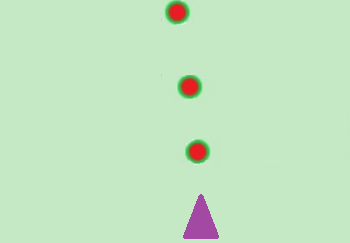
\includegraphics[width=2in]{img/rywalizacja1.png}
\captionsetup{justification=centering}
\captionof{figure}{Początek rywalizacji biegowej.}
\label{fig:rywalizacja1}
}
\end{table}%

\begin{table}[h!]
\parbox{\dimexpr\linewidth-6cm\relax}{\centering%
\captionsetup{justification=centering}
\captionof{table}{Ranking po „osiągnięciu” kolejnego punktu kontrolnego.}\label{table:rywalizacja2}
\begin{tabular}{|c|c|}
\hline
%\textbf{L.p.} & \textbf{Szerokość \newline geograficzna} & \textbf{Długość geograficzna} \\
 \begin{tabular}[c]{@{}c@{}}Zajmowana\\pozycja\end{tabular} & \begin{tabular}[c]{@{}c@{}}Użytkownik\end{tabular} \\
\hline
1 & Użytkownik B\\\hline
2 & Użytkownik A\\\hline
\rowcolor{GREEN}
3 & Bieżący użytkownik\\\hline
4 & Użytkownik C\\\hline
\end{tabular}
\label{tab:xt}}
\parbox{5cm}{%
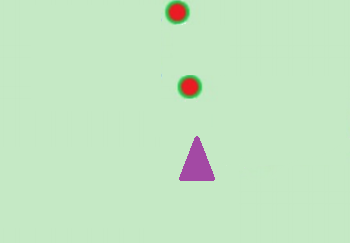
\includegraphics[width=2in]{img/rywalizacja2.png}
\captionsetup{justification=centering}
\captionof{figure}{Rywalizacja biegowa po osiągnięciu kolejnego punktu.}
\label{fig:rywalizacja2}
}
\end{table}%

Tak jak zostało wspomniane we wstępie do niniejszego rozdziału, użytkownik ma możliwość rywalizacji „ze samym sobą”, a więc oprócz próby obecnej w rankingu może znajdować się także próba biegacza dodana w czasie treningu odbytego wcześniej. Takie zjawisko może mieć jednak miejsce tylko w czasie trwania treningu. Oznacza to, że po jego zakończenia musi zajść jeden z następujących scenariuszy:
\begin {itemize}
\item{użytkownik nie odbył wcześniej treningu w ramach trasy - bieżąca próba jest zapisywana w systemie},
\item{użytkownik odbył wcześniej trening w ramach trasy, jego końcowy rezultat był lepszy niż w próbie bieżącej - bieżąca próba zostaje odrzucona},
\item{użytkownik odbił wcześniej trening w ramach trasy, jego końcowy rezultat był gorszy niż w próbie bieżącej - bieżąca próba zastępuje w systemie próbę poprzednią}.
\end{itemize}
\section{Informowanie użytkownika o rezultatach}
Podstawowym sposobem informowania biegacza jest wyświetlanie stanu treningu na ekranie urządzenia. Użytkownik ma do dyspozycji interaktywną mapę na której pokazana jest jego aktualna pozycja oraz wszystkie punkty kontrolne. Za każdym razem gdy następny w kolejności punkt kontrolny zostanie „osiągnięty”, zostaje on usunięty z mapy, aby użytkownik był świadom, że może udać się w kierunku kolejnego. Ponadto na ekranie wyświetlony jest ranking bieżącej rywalizacji biegowej. Przedstawia on czas osiągnięty na ostatnim punkcie kontrolnym oraz nazwy użytkownika wszystkich biegaczy, których próba zapisana jest w systemie. Miejsca w rankingu aktualizowane są za każdym razem gdy biegacz, który odbywa trening, osiągnie następny punkt kontrolny.

Biegacze często korzystają w czasie treningu z zestawu słuchawkowego. Wobec tego w celu zwiększenia immersji płynącej z wirtualnej rywalizacji, użytkownik informowany jest o rezultatach poprzez odtworzenie głosowych komunikatów. Za każdym razem gdy użytkownik „osiągnie” punkt kontrolny odtwarzana jest informacja:
\begin{itemize}
\item{\textbf{o aktualnie zajmowanej pozycji}, gdy pozycja zajmowana na właśnie „osiągniętym” punkcie kontrolnym jest taka sama jak na poprzednim punkcie kontrolnym},
\item{\textbf{o liczbie zdobytych pozycji}, gdy pozycja zajmowana na właśnie „osiągniętym” punkcie kontrolnym jest lepsza niż na poprzednim punkcie kontrolnym},
\item{\textbf{o liczbie utraconych pozycji}, gdy pozycja zajmowana na właśnie „osiągniętym” punkcie kontrolnym jest słabsza niż na poprzednim punkcie kontrolnym}.
\end{itemize}